\chapter{Application III: Fusion Plasma-Facing Components}
\label{ch:fusion-app}

The two preceding application chapters examined ion energy flux quantification in the low-temperature, low-heat-flux regimes of semiconductor processing and electric propulsion. This chapter turns to the opposite extreme: the divertor and first-wall surfaces of a magnetically confined fusion device, where the same sheath-transmitted ion energy flux $\Gamma_{E}$ that governs etch anisotropy or thruster grid erosion instead determines whether a plasma-facing component survives its operating campaign at all. A tokamak or stellarator confines a core plasma at tens of kilo-electron-volts, but essentially all exhaust power must cross a magnetized presheath and Debye-scale sheath before reaching a surface of finite thermal and erosion tolerance -- the same Bohm-constrained flux problem developed earlier, now at power densities one to four orders of magnitude larger, on materials that must survive $10^{4}$--$10^{5}$ pulses over a multi-year lifetime. This chapter surveys the power-exhaust problem, the SOL physics setting the delivered flux, the resulting erosion, melting, and tritium-retention consequences, present diagnostics and their limitations, and the case for a validated, non-intrusive flux diagnostic.

\section{The Divertor and First Wall: Heat and Particle Loads}

\subsection{The power-exhaust problem}

A burning-plasma tokamak must exhaust the fusion alpha-heating, auxiliary, and ohmic power through a narrow annulus of open field lines connecting the plasma to material surfaces:
\begin{equation}
P_{\mathrm{SOL}} = P_{\mathrm{heat}} - P_{\mathrm{rad}}^{\mathrm{core}},
\label{eq:powerbalance}
\end{equation}
where $P_{\mathrm{heat}}$ is the total input power and $P_{\mathrm{rad}}^{\mathrm{core}}$ the power radiated volumetrically from the confined plasma \cite{ref0093}. $P_{\mathrm{SOL}}$ is deposited on divertor targets and, to a lesser degree, the first wall: a few to tens of megawatts in present-day devices, order $\SI{100}{MW}$ in ITER, with compact high-field pilot plants facing a more severe exhaust problem despite being physically smaller. This power spreads over a wetted area set by the SOL width, determined by the edge transport physics of Section~\ref{sec:sol-physics} rather than divertor design freedom. If that width remains narrow at reactor scale, peak heat flux at the strike point becomes the single most constraining engineering parameter of the device \cite{ref0581}.

\subsection{Divertor geometry and the two-point model}

The divertor is a specialised region of the first wall, magnetically connected to the plasma edge via a poloidal field null (the X-point), onto which most of the exhausted power and particle flux is directed. It localises the highest loads onto replaceable, cooled plates, pumps helium ash and recycling gas, and reduces the temperature and heat flux at the strike point through long connection length and volumetric dissipation. The standard reduced description, the two-point model, relates upstream conditions ($u$) to the target ($t$) through parallel pressure balance,
\begin{equation}
n_{u} T_{u} \simeq n_{t} T_{t} \left(1 + M_{t}^{2}\right),
\label{eq:twopoint-pressure}
\end{equation}
and parallel power balance, where conducted heat flux relates to the temperature gradient by the Spitzer--Härm form
\begin{equation}
q_{\parallel} = -\kappa_{0} T_{\mathrm{e}}^{5/2} \frac{\mathrm{d}T_{\mathrm{e}}}{\mathrm{d}s},
\label{eq:spitzer}
\end{equation}
with $\kappa_{0}$ the classical electron parallel heat conductivity coefficient and $s$ the field-line coordinate. At low target temperature and high density this closure breaks down: the electron mean free path becomes comparable to the gradient scale length, and non-local kinetic effects modify the effective conductivity and the distribution function reaching the sheath edge, affecting the electron temperature of Section~\ref{sec:sheath-heat}. At the target, the plasma terminates on a magnetized presheath (Chodura layer) and Debye-scale sheath, so the armour flux is set by the local sheath-edge density $n_{\mathrm{i}}$, temperatures $T_{\mathrm{e}}$, $T_{\mathrm{i}}$, and magnetic incidence angle -- not upstream core parameters.

\subsection{Steady-state and transient load specifications}

Two load categories must be specified for design: the steady-state (inter-pulse) flux, set by the time-averaged $P_{\mathrm{SOL}}$ and SOL width, typically \SI{5}{}--\SI{20}{MW.m^{-2}} at the strike point, peaking where geometry departs from axisymmetry; and the transient load from ELMs, disruptions, vertical displacement events, and runaway-electron strikes, where a large fraction of stored plasma energy is deposited on a millisecond timescale over an area much smaller than the steady-state wetted area. Transients dominate the erosion and fatigue budget despite occupying little operating time. Table~\ref{tab:load-categories} summarises the distinction.

\begin{table}[htbp]
\centering
\caption{Illustrative, order-of-magnitude comparison of steady-state and transient plasma-facing-component load categories. Values are representative design ranges, not measurements from a specific device.}
\label{tab:load-categories}
\begin{tabular}{@{}lll@{}}
\toprule
Characteristic & Steady-state / inter-ELM & Transient (ELM, disruption) \\
\midrule
Duration & continuous & \SI{0.1}{}--\SI{5}{ms} \\
Peak heat flux & \SI{5}{}--\SI{20}{MW.m^{-2}} & \SI{e2}{}--\SI{e4}{MW.m^{-2}} \\
Dominant damage mode & gradual erosion, fatigue & melting, cracking, ablation \\
Governing flux quantity & $\Gamma_{E}$ time-averaged & energy density per pulse \\
Primary diagnostic need & continuous monitoring & pulse-resolved capture \\
\bottomrule
\end{tabular}
\end{table}

\section{Edge and Scrape-Off-Layer Physics Delivering Flux to Surfaces}
\label{sec:sol-physics}

\subsection{The scrape-off layer as a magnetised presheath--sheath system}

The scrape-off layer is the region of open field lines between the last closed flux surface and the material wall: an extended magnetised presheath in which particles and energy transport toward the divertor targets, while a thin electrostatic sheath at the surface enforces quasineutrality breakdown and accelerates ions to it. The generalized magnetized Bohm criterion, $u_{\parallel} \geq u_{\mathrm{B}}\sin\alpha$ at grazing angle $\alpha$, together with the more restrictive Chodura condition at the presheath's outer edge, sets the boundary condition coupling the SOL solution to the sheath-transmitted flux. The Bohm speed retains its familiar form,
\begin{equation}
u_{\mathrm{B}} = \sqrt{\frac{k_{B}\left(T_{\mathrm{e}} + T_{\mathrm{i}}\right)}{m_{\mathrm{i}}}},
\label{eq:fusion_bohm}
\end{equation}
and the local Debye length,
\begin{equation}
\lambda_{\mathrm{D}} = \sqrt{\frac{\varepsilon_{0} k_{B} T_{\mathrm{e}}}{n_{\mathrm{e}} e^{2}}},
\label{eq:fusion_debye}
\end{equation}
remains microscopic compared to both the ion Larmor radius and the SOL width, so the sheath is a thin layer nested inside the much larger magnetized presheath and SOL flux tube. What distinguishes the fusion edge from processing-plasma sheaths treated earlier is not the local sheath physics -- identical in kind -- but the anisotropic, magnetically structured transport that sets the density, temperature, and ion distribution function $f_{\mathrm{i}}(v)$ arriving at the sheath entrance.

\subsection{Parallel transport and the heat-flux width}

The width of the SOL heat-flux channel, $\lambda_{q}$, is the single parameter converting $P_{\mathrm{SOL}}$ into a peak surface heat flux, and its scaling to reactor-relevant, high-field, small-machine devices has been a central open question in edge physics. The parallel heat-flux profile at the target is well described empirically by the Eich fit function, convolving an exponential decay of length $\lambda_{q}$ with a Gaussian broadening of width $S$ representing near-SOL transport:
\begin{equation}
q_{\parallel}(s) = \frac{q_{0}}{2}\exp\!\left[\left(\frac{S}{2\lambda_{q}}\right)^{2} - \frac{s}{\lambda_{q} f_{x}}\right] \operatorname{erfc}\!\left(\frac{S}{2\lambda_{q}} - \frac{s}{S f_{x}}\right) + q_{\mathrm{BG}},
\label{eq:eich}
\end{equation}
where $s$ is the distance from the strike point mapped to the outer midplane, $f_{x}$ the flux expansion factor, and $q_{\mathrm{BG}}$ a broad background component. In the limit $S \to 0$, Eq.~\eqref{eq:eich} reduces to $q_{\parallel}(s) = q_{0}\exp(-s/\lambda_{q})$, plotted schematically in Figure~\ref{fig:sol-heatflux}. Multi-machine regression finds $\lambda_{q}$ scales unfavourably with plasma current and only weakly with machine size, confirmed by empirical fits and gyrokinetic simulations extrapolated to ITER. The near-SOL profile can also bifurcate into a narrow, high-amplitude feature superposed on the broader channel, requiring active suppression in target design. Because $\lambda_{q}$ sets the sheath-edge density and hence $\Gamma_{E}$ through Eq.~\eqref{eq:sheath-flux}, its uncertainty propagates directly into peak divertor loading.

\begin{figure}[htbp]
\centering
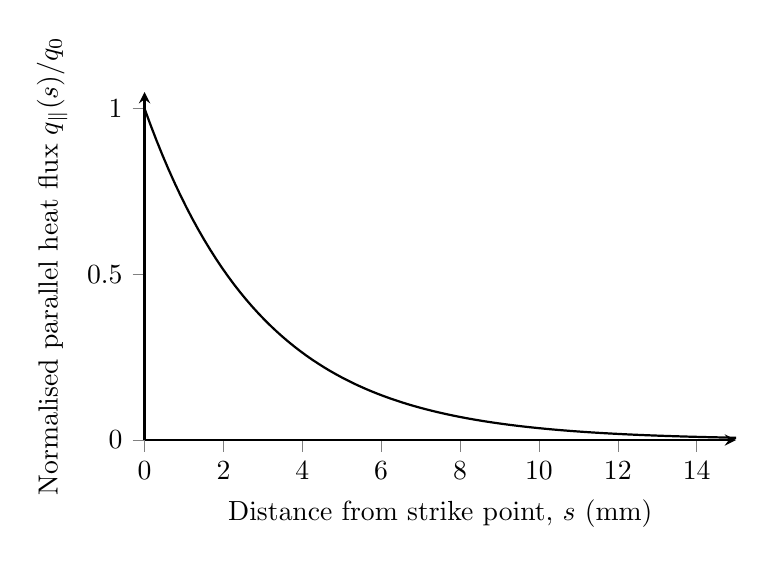
\begin{tikzpicture}
\begin{axis}[
 width=0.75\textwidth,
 height=6cm,
 xlabel={Distance from strike point, $s$ (mm)},
 ylabel={Normalised parallel heat flux $q_{\parallel}(s)/q_{0}$},
 domain=0:15,
 samples=100,
 axis lines=left,
 ymin=0,
 ymax=1.05,
 xmin=0,
 xmax=15,
 thick,
 tick align=outside,
]
\addplot[black, thick] {exp(-x/3)};
\end{axis}
\end{tikzpicture}
\caption{Schematic exponential scrape-off-layer parallel heat-flux profile, $q_{\parallel}(s) = q_{0}\exp(-s/\lambda_{q})$, the $S \to 0$ limit of Eq.~\eqref{eq:eich}, drawn for an arbitrary decay length $\lambda_{q} = \SI{3}{mm}$. The curve illustrates the functional form only; it is not measured data.}
\label{fig:sol-heatflux}
\end{figure}

\subsection{Cross-field transport and intermittency}

Parallel transport is only part of the picture: cross-field turbulent transport redistributes particles and heat across the SOL and carries a fraction of the exhaust directly to the first wall, dominated by coherent, filamentary structures ("blobs") that detach intermittently from the edge. Characterisation on machines such as MAST shows the resulting profiles are strongly non-Gaussian and intermittent, with filament statistics setting the effective SOL width felt by the far first wall even where Eq.~\eqref{eq:eich} predicts negligible flux \cite{ref0600}. Magnetic fluctuations and neutral recycling further modify the diffusivity and must be retained in turbulence codes projecting SOL behaviour to reactor parameters \cite{ref0605}. Consequently, the first-wall flux fluctuates rather than remaining steady, with statistics a machine-protection diagnostic must resolve rather than time-average \cite{ref0611}.

\subsection{Parallel flows, drifts, and poloidal asymmetry}

The SOL flux delivered to a divertor target is not poloidally symmetric even for an up-down symmetric configuration, because $\mathbf{E}\times\mathbf{B}$ and diamagnetic drifts superpose a net parallel Mach flow on the conduction-convection picture of Eq.~\eqref{eq:spitzer}. This flow's direction and magnitude depend sensitively on the sign of the toroidal field and plasma current, producing systematic in/out and up/down target-flux asymmetries a one-dimensional two-point model cannot capture. The interchange instability seeding cross-field turbulence has been analysed as a magnetised analogue of Rayleigh--B\'{e}nard convection, with unfavourable outboard-midplane curvature the destabilising factor -- explaining why the outboard SOL is systematically more turbulent and broader than the inboard SOL. This asymmetry is not a second-order correction: a single witness location can mis-estimate the peak-loading flux unless the diagnostic provides toroidally and poloidally resolved coverage.

\subsection{Detachment and volumetric power and momentum loss}

At sufficiently high target density and low temperature, the plasma can enter a "detached" regime in which volumetric processes -- ionisation, excitation, charge exchange, and recombination -- dissipate a substantial fraction of parallel power and momentum flux before reaching the surface, decoupling target pressure from the upstream pressure of Eq.~\eqref{eq:twopoint-pressure}. Detachment is the primary strategy for reducing peak heat flux to tolerable levels; reduced 1D models extending the two-point model with atomic source/sink terms reproduce its essential features. It is not passive or automatically stable: it must be actively controlled against insufficient detachment (heat flux too high) or excessive detachment (extinguishing the divertor plasma, compromising impurity control), motivating the real-time flux diagnostics of Section~\ref{sec:relevance}.

\section{Erosion, Melting, Tritium Retention, and Component Lifetime}

\subsection{Sheath-transmitted power and the erosion problem}
\label{sec:sheath-heat}

The ion energy flux delivered through the sheath to the target surface is the product of the particle flux and the mean energy transported per ion-electron pair, expressed via the sheath heat-transmission coefficient $\gamma$:
\begin{equation}
\Gamma_{E} = \gamma\, k_{B} T_{\mathrm{e}}\, n_{\mathrm{i}} u_{\mathrm{B}} \sin\alpha,
\label{eq:sheath-flux}
\end{equation}
with $n_{\mathrm{i}} u_{\mathrm{B}}\sin\alpha$ the Bohm-limited particle flux normal to the surface. The coefficient decomposes into ion and electron contributions,
\begin{align}
\gamma_{\mathrm{i}} &\simeq 2 + \frac{1}{2}\frac{m_{\mathrm{i}} u_{\mathrm{B}}^{2}}{k_{B} T_{\mathrm{e}}} \approx 2.5, \\
\gamma_{\mathrm{e}} &\simeq \frac{2}{1-\delta} - \ln\!\left[(1-\delta)\sqrt{\frac{2\pi m_{\mathrm{e}}}{m_{\mathrm{i}}}\left(1+\frac{T_{\mathrm{i}}}{T_{\mathrm{e}}}\right)}\right],
\label{eq:fusion_gamma_e}
\end{align}
where $\delta$ is the target's secondary-electron emission coefficient, so $\gamma = \gamma_{\mathrm{i}} + \gamma_{\mathrm{e}}$ typically evaluates to $6$--$8$ for divertor-relevant deuterium plasmas on low-emission tungsten. Secondary electron emission is not a mere correction: at oblique incidence and low temperature it can drive a transition toward a space-charge-limited or inverted sheath that changes $\gamma$ substantially, an effect that must be treated self-consistently rather than as a fixed constant. Equation~\eqref{eq:sheath-flux} is thus the direct fusion analogue of the ion energy flux relation applied elsewhere in this monograph, at power densities four to six orders of magnitude larger.

\subsection{Physical erosion and net erosion balance}

The eroded surface undergoes physical sputtering with an energy- and angle-dependent yield $Y(E,\theta)$ \cite{ref0143,ref0144}, giving a local gross erosion rate
\begin{equation}
\dot{d}_{\mathrm{ero}} = \frac{m_{\mathrm{atom}}}{\rho}\, Y(E,\theta)\, \Gamma_{\mathrm{i}},
\label{ch18-eq:erosion-rate}
\end{equation}
with $m_{\mathrm{atom}}$ the mass of one target atom and $\rho$ the material density. Because a substantial fraction of sputtered atoms are promptly ionised and returned to the surface by the same sheath field, the quantity determining lifetime is not gross erosion but the net balance of erosion and local redeposition. Studies of full-tungsten divertor tokamaks show this gross-to-net ratio can differ by an order of magnitude between locations, so gross-erosion yield curves alone give pessimistic lifetime projections unless redeposition is validated against migration experiments \cite{ref0593}. Melting is a further, non-sputtering channel: past the melting point, hydrodynamic melt-layer motion driven by $\mathbf{J}\times\mathbf{B}$ forces, surface tension gradients, and plasma pressure can displace material well beyond sputtering alone \cite{ref0176}.

\subsection{Transient loads, melting, and fracture}

Because transient events deposit energy on millisecond timescales too short for thermal diffusion to equilibrate through the bulk armour, the surface temperature rise for a semi-infinite solid subject to a heat-flux pulse of duration $\tau$ is
\begin{equation}
\Delta T_{\mathrm{surf}}(\tau) \approx \frac{2 q_{0}}{\sqrt{\pi}}\,\sqrt{\frac{\tau}{k \rho c_{p}}},
\label{eq:transient-temp}
\end{equation}
with $k$, $\rho$, $c_{p}$ the thermal conductivity, density, and specific heat of the armour. This explains why ELM and disruption transients, despite their short duration, are disproportionately damaging: the factor $q_{0}\sqrt{\tau}$ can exceed the melting or recrystallisation threshold of tungsten armour even when time-integrated energy density is modest, while repeated sub-melting cycling separately drives fatigue crack growth. High-heat-flux qualification campaigns on ITER-type tungsten monoblocks have quantified both the crack-initiation threshold and the progressive degradation of thermal performance with pulse count. Slow, mitigated-disruption transients, whose thermal quench stretches over several milliseconds, populate an intermediate regime whose damage cannot be interpolated between the inter-ELM and fastest-transient limits, since melt-layer and vapour-shielding physics differ qualitatively \cite{ref0176}. Runaway-electron strikes are a still more localised and severe transient, capable of melting or vaporising armour over areas far smaller than the ELM footprint.

\subsection{Tritium retention and fuel inventory}

For a deuterium-tritium device, a further consequence of the same flux driving erosion is fuel retention within plasma-facing components and redeposited material. Incident tritium implants to a depth set by the ion range at impact energy $E \sim \gamma_{\mathrm{i}} k_{B} T_{\mathrm{e}}$; a fraction is trapped at material defects, grain boundaries, and, most significantly, within re-deposited layers that grow wherever net erosion is negative. The retained fuel inventory obeys a balance of the schematic form
\begin{equation}
\frac{\mathrm{d}N_{\mathrm{T}}}{\mathrm{d}t} = f_{\mathrm{trap}}\,\Gamma_{\mathrm{T}}\,A_{\mathrm{wetted}} - \dot{N}_{\mathrm{T}}^{\mathrm{release}},
\label{eq:tritium}
\end{equation}
where $f_{\mathrm{trap}}$ is an effective trapping fraction (dependent on surface temperature, microstructure, and redeposition rate), $\Gamma_{\mathrm{T}}$ the tritium particle flux at wetted area $A_{\mathrm{wetted}}$, and $\dot{N}_{\mathrm{T}}^{\mathrm{release}}$ thermal or isotope-exchange release. Because regulatory limits on in-vessel tritium inventory are a hard operational constraint, an accurate, spatially resolved measurement of $\Gamma_{\mathrm{T}}$ is licensing-relevant -- made difficult by co-deposition zones, precisely the regions of highest net erosion of Section~\ref{sec:erosion-net}, hard to predict from first principles. The strong sensitivity of $f_{\mathrm{trap}}$ to surface temperature further couples retention to the transient heat-load problem of Eq.~\eqref{eq:transient-temp}, since ELM and disruption heating can drive both additional trapping and thermally activated release.

\subsection{Lifetime budgeting}
\label{sec:erosion-net}

Combining Eqs.~\eqref{ch18-eq:erosion-rate}--\eqref{eq:transient-temp}, an armour tile of thickness $d_{0}$ subject to a steady-state net erosion rate $\dot{d}_{\mathrm{net}}$ and a per-pulse melting probability $p_{\mathrm{melt}}$ has an expected operational lifetime bounded above by
\begin{equation}
t_{\mathrm{life}} \lesssim \min\left(\frac{d_{0}}{\dot{d}_{\mathrm{net}}},\ \frac{1}{p_{\mathrm{melt}}\, f_{\mathrm{pulse}}}\right),
\label{eq:lifetime}
\end{equation}
where $f_{\mathrm{pulse}}$ is the transient-event repetition rate. High-heat-flux qualification facilities determine the coefficients entering Eq.~\eqref{eq:lifetime} under controlled, repeatable conditions before a design is accepted for installation \cite{ref0586,ref0588}. A component that erodes safely under plasma load can still fail catastrophically if its coolant channel is separately driven into critical heat flux, coupling the erosion problem to a conjugate thermal-hydraulic design problem not typical of processing-plasma or propulsion contexts.

\section{Edge Diagnostics and Their Limitations}

\subsection{Intrusive probe diagnostics}

Langmuir and retarding-field energy analyser (RFEA) probes remain the most direct means of measuring local plasma density, temperature, and ion energy distribution at the divertor target and near-SOL, with RFEA measurements used to infer SOL ion temperature at the strike point \cite{ref0610}. The limitation is structural: any probe inserted into the SOL is itself a small plasma-facing component, subject to the same sheath, erosion, and heat-load constraints analysed in Section~3, and it perturbs the local plasma by drawing current. Probes at the highest-flux regions cannot be left in place continuously without being destroyed or contaminating the measurement with their own erosion products; they are therefore restricted to lower-flux locations, brief excursions, or sacrificial configurations, none of which give the continuous coverage machine protection requires.

\subsection{Non-intrusive optical, scattering, and interferometric diagnostics}

Thomson scattering provides a genuinely non-intrusive, spatially and (with fast lasers) temporally resolved measurement of electron density and temperature, and divertor/edge Thomson systems continue to be built into new machines for continuous coverage that probes cannot provide \cite{ref0383}. Microwave interferometry provides a complementary, non-perturbing, line-integrated measurement of edge electron density \cite{ref0399}. Both techniques, however, measure the electron-fluid moments $n_{\mathrm{e}}$ and $T_{\mathrm{e}}$ rather than $\Gamma_{E}$ directly; converting either into a flux estimate requires an auxiliary assumption -- typically the Bohm criterion of Eq.~\eqref{eq:fusion_bohm} with an assumed or separately measured $T_{\mathrm{i}}$ and $\gamma$ -- precisely the closure this monograph validates. Edge spectroscopy can, in favourable cases, independently estimate $T_{\mathrm{i}}$, but requires a collisional-radiative model and line-of-sight integration; the same fluctuation diagnostics essential to characterising Section~\ref{sec:sol-physics}'s intermittent transport again report fluctuations rather than calibrated energy flux \cite{ref0611}.

\subsection{Thermal and calorimetric inference}

Infrared thermography and embedded thermocouple or calorimeter arrays measure the consequence of the incident flux -- the resulting temperature rise -- rather than the flux itself, requiring an inverse heat-conduction solution to recover the incident heat-flux profile \cite{ref0175}, well-posed only given accurate thermal properties, surface emissivity, and geometric shadowing, all of which evolve with accumulated damage. Critically, these methods report the total absorbed power density -- summing ion kinetic and potential (recombination) energy, transmitted electron thermal flux, and radiative loading -- without separating these channels, so they cannot isolate $\Gamma_{E}$, which governs sputtering and tritium retention, from contributions that neither erode the surface nor retain fuel.

\subsection{The common shortfall}

Across all three families, the same gap recurs: probe-based methods measure ion energy flux directly but cannot survive, or operate continuously, at the highest-flux locations and times that matter most; non-intrusive optical and scattering methods survive and operate continuously but measure plasma-fluid moments requiring an unvalidated closure; and thermal/calorimetric methods measure the flux's net consequence non-intrusively but cannot resolve its composition. Table~\ref{ch18-tab:diagnostics} summarises the trade-off.

\begin{table}[htbp]
\centering
\caption{Qualitative comparison of principal edge and divertor diagnostic families against criteria relevant to ion energy flux quantification. Entries are qualitative assessments drawn from the literature, not benchmarking data.}
\label{ch18-tab:diagnostics}
\begin{tabular}{@{}lccc@{}}
\toprule
Diagnostic & Non-intrusive & Direct $\Gamma_{E}$ access & Survives peak transient \\
\midrule
Langmuir / RFEA probe \cite{ref0610} & no & yes & no \\
Thomson scattering \cite{ref0383} & yes & no (requires closure) & yes \\
Microwave interferometry \cite{ref0399} & yes & no (density only) & yes \\
Edge spectroscopy & yes & partial ($T_{\mathrm{i}}$ only) & yes \\
IR thermography / calorimetry \cite{ref0175} & yes & no (unresolved channels) & yes \\
\bottomrule
\end{tabular}
\end{table}

\section{Relevance of a Validated Non-Intrusive Flux Diagnostic to Fusion Viability}
\label{sec:relevance}

\subsection{Machine protection and real-time control}

Modern tokamak operation increasingly relies on real-time control systems to regulate the divertor state -- triggering impurity seeding or gas puffing to maintain detachment, adjusting heating power near operational limits, and, facing an imminent disruption, triggering mitigation systems. Each control loop needs a real-time estimate of the divertor flux, or the margin before a threshold such as Eq.~\eqref{eq:transient-temp} is reached. A non-intrusive diagnostic independently validated against the true $\Gamma_{E}$ -- rather than an unverified closure of the kind flagged in Section~4.4 -- would let such loops act on a meaningful quantity rather than an uncertain proxy, particularly for detachment control, where the models of Section~2.4 are themselves approximations benefiting from independent validation.

\subsection{Materials qualification and lifetime prediction}

The erosion, melting, and tritium-retention models of Section~3 all take the local ion energy and particle flux as primary input, so every step to a lifetime prediction -- Eqs.~\eqref{ch18-eq:erosion-rate}, \eqref{eq:transient-temp}, \eqref{eq:tritium} -- inherits whatever uncertainty exists in the flux itself. High-heat-flux qualification facilities validate component response under controlled loading \cite{ref0586,ref0588}, but that validation's fidelity to reactor operation depends on how accurately the in-vessel flux during a real discharge is known, particularly during the transients dominating the erosion and fatigue budget. A validated non-intrusive diagnostic resolving $\Gamma_{E}$ throughout a discharge -- including during ELMs and a disruption thermal quench, precisely the events probes cannot survive -- would close the loop between laboratory qualification and in-vessel performance, letting gross-versus-net erosion balances be tracked directly rather than inferred post-mortem \cite{ref0593}.

\subsection{Extrapolation to steady-state burning-plasma devices}

The case for such a diagnostic is strongest precisely where probe-based measurement is least viable: in steady-state or long-pulse burning-plasma devices and compact, high-power-density pilot plants, where the divertor operates continuously at high heat flux for durations far exceeding what any inserted probe could survive. There, the non-intrusive diagnostic families of Section~4.2 are the only ones capable of continuous operation, yet also the ones whose connection to the flux of interest is least direct. A framework demonstrating, with validation against direct measurement in accessible regimes, how a non-intrusive observable maps onto the true sheath-transmitted flux -- rather than relying on untested extrapolation of a fluid closure -- is a prerequisite for extending confident heat-load and lifetime prediction to the steady-state operation on which fusion power plant economics depend.

\section{Summary}

The divertor and first wall of a magnetically confined fusion device must absorb essentially the entire exhaust power of the plasma through the same sheath-transmitted ion energy flux mechanism examined throughout this monograph, but at power densities and fluences that place component lifetime, rather than process yield or thrust efficiency, at stake. The SOL transport physics reviewed here -- parallel conduction and its kinetic corrections, the heat-flux-width scaling, cross-field intermittent transport, and detachment -- together set the density, temperature, and distribution function delivered to the sheath at the target, from which Eq.~\eqref{eq:sheath-flux} yields the flux governing erosion, transient melting, and tritium retention. Present-day edge diagnostics resolve this picture only partially: probe-based instruments access the flux directly but cannot survive the highest-flux locations and transient events that matter most, while non-intrusive optical, scattering, and thermal methods survive but either require an unvalidated closure or cannot resolve the composition of the measured load. A validated, non-intrusive ion energy flux diagnostic of the kind developed here directly addresses this shortfall: real-time divertor and disruption control, closing the loop between laboratory qualification and in-vessel performance, and extrapolating heat-load and lifetime prediction to the steady-state burning-plasma devices on which fusion power's practical viability depends.
